\section{Identification of a Soft Robot}
\label{sec:experiment}

To demonstrate \David{This comes back to the contribution.  ``In this work, we propose to apply this process to a soft robotic system and evaluate its performance to other nonlinear system ...} the performance of the technique outlined in Section \ref{sec:theory}, we applied it to a continuously deformable soft robot arm and compared the resulting model to those generated by other nonlinear system identification techniques.
\David{In the following, we explain in detail the used robotic hardware, experimental setup, measurement proces, ...}This section describes the composition of the robot and recount the setup, measurement, and data pre-proccessing involved in the system identification process.
% We also describe how the accuracy of the resulting model was calculated in terms of the root-mean-square error of its state predictions.
In the Results section... \David{Why mention results already here?}

\subsection{Hardware description}

The soft robot used in this experiment consisted of three pneumatically driven McKibben actuators (also known as Pneumatic Artificial Muscles or PAMs) adhered together by latex rubber and connected to a common base mount \David{on one and and to an} end effector \David{on the other} (see Fig. \ref{fig:flaccy}).
During the trials, the pressure inside each actuator was varied using a pneumatic pressure regulator (Enfield TR-010-g10-s), and the displacement and velocity of the end effector was measured at $60 \text{Hz}$ using a commercial motion capture system (Phase Space Impulse X2E).

%% state space representation of model
\David{Try to use more declarative language.  We have discussed this in the past.  Other people do a lot of different things (and might disagree in your notion of primary interest), but you can simply say what your interest is: ``Our declared control goal for this setup is to dynamically control the kinematic motion of ...} With robotic manipulators, it is often of primary interest to dynamically control the motion of the end effector.
\David{To this end, we chose...} It is convenient then, to choose a state representation of the system which is capable of describing the dynamics of the end effector as an ODE.
For this reason, we chose to represent the state of our soft robot as the position and velocity of the end effector with respect to a global coordinate frame, as shown in Fig. \ref{fig:flaccy}
\begin{align}
    \vec{x} &= \mtx{ x_1 & x_2 & x_3 & \dot{x_1} & \dot{x_2} & \dot{x_3} }^T
    \label{eq:state}
\end{align}

\subsection{Randomized control input}

to generate a representative sampling of the system's behavior over its entire operation range, a randomized input was applied.
The control input into the system $\uv$ was a set of three $0-10 \text{V}$ \Ram{This is bad notation. $\uv(t)$ is the control input at time $t$. $\uv$ is the control input. Please be careful about these kinds of things as they tend to confuse the reader.} signals into the pressure regulators corresponding to actuator pressures of $\approx 0-140 \text{ kPa}$
\aln{
    \uv (t) &= \mtx{ u_1 (t) & u_2 (t) & u_3 (t) }^T,   && u_i \in [0,10]
}
\David{I don't follow the indices.  also, don't you have a special notation for vectors?}
Before each trial, a $3 \times 1000$ table $\Upsilon$ of uniformly distributed random numbers between zero and ten was generated to be used as an input lookup table.
Each control input was smoothly varied between elements in consecutive columns of the table over a transition period $T_u$, with a time offset of $T_u / 3$ between each of the three control signals
\aln{
    u_i (t) &= \frac{(\Upsilon_{i,k+1} - \Upsilon_{i,k})}{T_u} \left( t + \frac{(i-1) T_u}{3} \right) + \Upsilon_{i,k}
}
where $k = \text{floor}\left( {t} / {T_u} \right)$ is the current index into the lookup table at time $t$ (see Fig. \ref{fig:randInput}).

%% Figure: Randomized Inputs
\begin{figure}
    \centering
    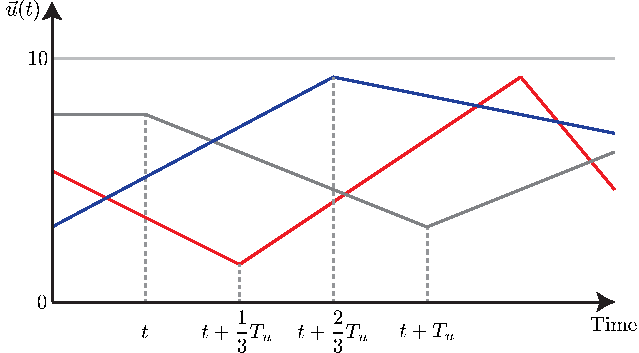
\includegraphics[width=\linewidth]{figures/randInput3dim.pdf}
    \caption{Caption: Randomized control inputs \David{I would add the dotted line at t+4/3T.}}
    \label{fig:randInput}
\end{figure}

% The measured output of the system $\vec{y}(t)$ was the $xyz$ position of the end effector. Numerical derivatives were taken between sampling points to define the velocity of the end effector
% \aln{
%     \vec{y}(t) = \mtx{x(t) & y(t) & z(t)}^T
% }

\subsection{Data collection}

Data collection proceeded in 5 trials. The specific testing parameters for each trial can be found in Table \ref{tab:trialParams}.

%% TABLE: Trial parameters
\begin{table}[h]
    \centering
    \caption{Data Collection Parameters}
    \begin{tabular}{|c||c|c|}
        \hline
         & $\bm{T_u}$ \textbf{(s)} & \textbf{Length (min)} \\
        \hline
         Trial 1 & 3 & 40:06 \\
         Trial 2 & 3.5 & 31:26 \\
         Trial 3 & 4 & 8:16 \\
         Trial 4 & 5 & 26:09 \\
         Trial 5 & 5 & 28:38 \\
         Trial 6 & 8 & 31:35 \\
        \hline
    \end{tabular}
    \label{tab:trialParams}
\end{table}

After collecting data, raw position and velocity measurements were put through a moving average filter with window size of $1$s to reduce noise, then sampled uniformly with a period $T_s = 0.02 \text{s}$.
Sampled velocity measurements were put through a second moving average filter with window size of $1$s, due to the higher noise content of the velocity signal.
%% Partitioning of trail data into training and validation sets
The time-series data from each trail was partitioned into training and validation sets. 
Three validation sets lasting 10 seconds each were extracted from each trial and the remainder of the trial data was used for training.

%% FIGURE: Showing what flaccy looks like
\begin{figure}
    \centering
    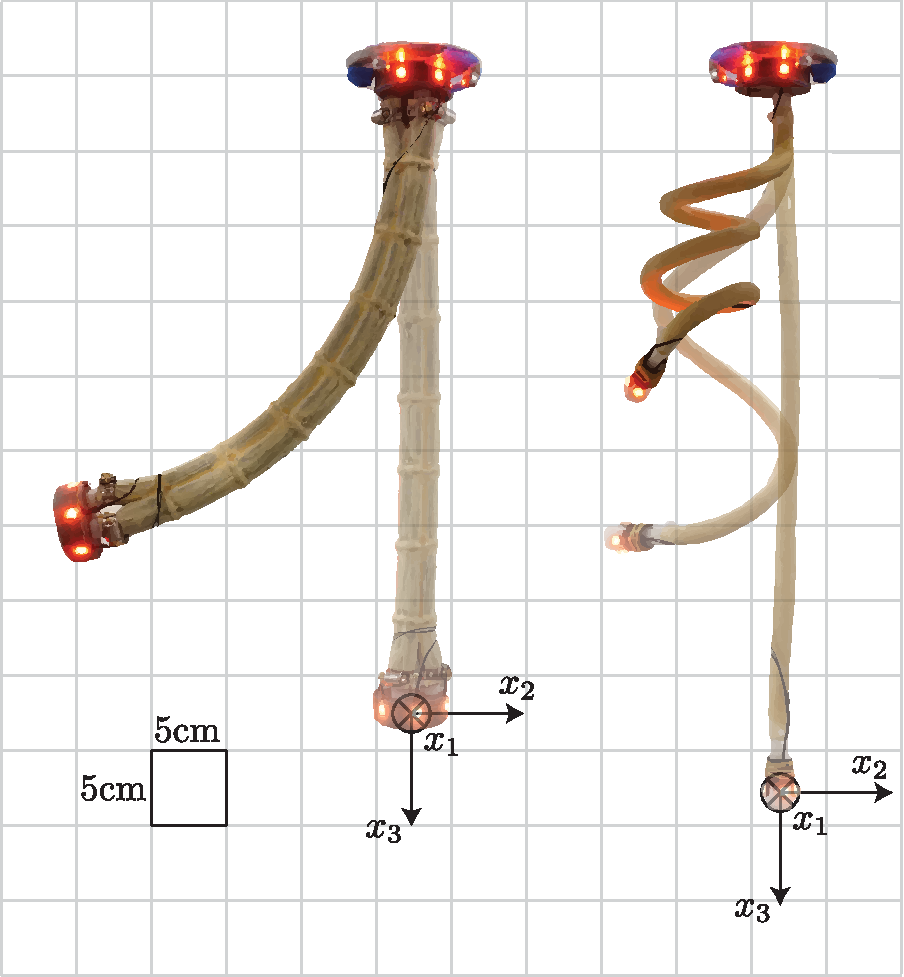
\includegraphics[width=\linewidth]{figures/robotsDiagram_v2.pdf}
    \caption{PLACEHOLDER: This final version of this diagram needs to show the scale of flaccy, the maximum deformation, and the location and orientation of the global coordinate frame.}
    \label{fig:flaccy}
\end{figure}